\section{结果图表与可视化分析}

\subsection{主实验结果汇总}

结合当前仓库实际运行结果，主实验的分类表现可整理如下表。本文严格区分 holdout 与 CV 口径，并以日志文件中的可复现结果为准。

\begin{table}[H]
\centering
\caption{主实验结果汇总（当前日志版本）}
\begin{tabular}{lccc}
\toprule
方法 & Accuracy/Balanced Accuracy/Macro-F1 & 评估口径 & 结果特点 \\
\midrule
RNA-only & 0.875/0.8889/0.8857 & holdout & 单模态强基线 \\
Concat & 0.875/0.8889/0.8857 & holdout & 实现简单、稳定 \\
MOFA & 0.875/0.8889/0.8857 & holdout & 可解释潜力较好 \\
Stacking & $0.7940\pm0.1648$/$0.7963\pm0.1693$/$0.7899\pm0.1695$ & 5-fold CV & 波动较大、需进一步调参 \\
\bottomrule
\end{tabular}
\end{table}

从当前结果可以看出，单次 holdout 与严格 CV 的结论存在差异。前者显示三种主线方案表现接近，后者显示 stacking 在现参数下稳定性不足。这一差异提示：后续应优先报告重复 CV/外部验证结果，而非仅依赖单次切分高分。

\subsection{消融实验结果汇总}

消融实验结果更能说明各模块的必要性。当前结果如下：

\begin{table}[H]
\centering
\caption{消融实验结果汇总}
\begin{tabular}{lccc}
\toprule
消融设置 & Accuracy & 影响对象 & 解读 \\
\midrule
去甲基化 & 0.75 & 数据模态 & 单一 RNA 可用但不优 \\
去 RNA & 0.75 & 数据模态 & 甲基化可提供补充信息 \\
不做特征选择 & 0.25 & 预处理策略 & 高维噪声显著干扰模型 \\
\bottomrule
\end{tabular}
\end{table}

其中“不做特征选择”表现最差，说明高维噪声对当前任务影响显著，也从侧面证明高方差筛选并非可有可无，而是分类稳定性的关键步骤。

\subsection{分类报告的类别级差异}

从分类报告看，不同类别的 precision、recall 与 F1-score 存在明显差异。一般来说，样本量较少的类别更容易表现出较大的波动，这与当前实验样本规模有限有关。对于乳腺癌亚型任务而言，Basal 和 HER2 类别往往在生物学上更具特殊性，但在统计上可能样本更少，因此分类器更容易受到数据划分影响。

这也提示后续分析中需要进一步使用混淆矩阵和重复实验来验证结论的稳健性。若仅依据单次 Accuracy，很容易忽略“某一类被很好识别，而另一类识别失败”的情况。因此，在研究报告中应将类别级别的指标与整体 Accuracy 并列展示。

\subsection{基于真实日志的核心可视化}

为保证结果图与实验日志严格一致，本文新增一组由 \texttt{outputs/logs/summary.csv} 自动生成的图表（脚本：\texttt{scripts/plot\_experiment\_results.py}）。该组图表用于正文主证据展示，避免模拟数据图混入结论链条。

\begin{figure}[H]
\centering
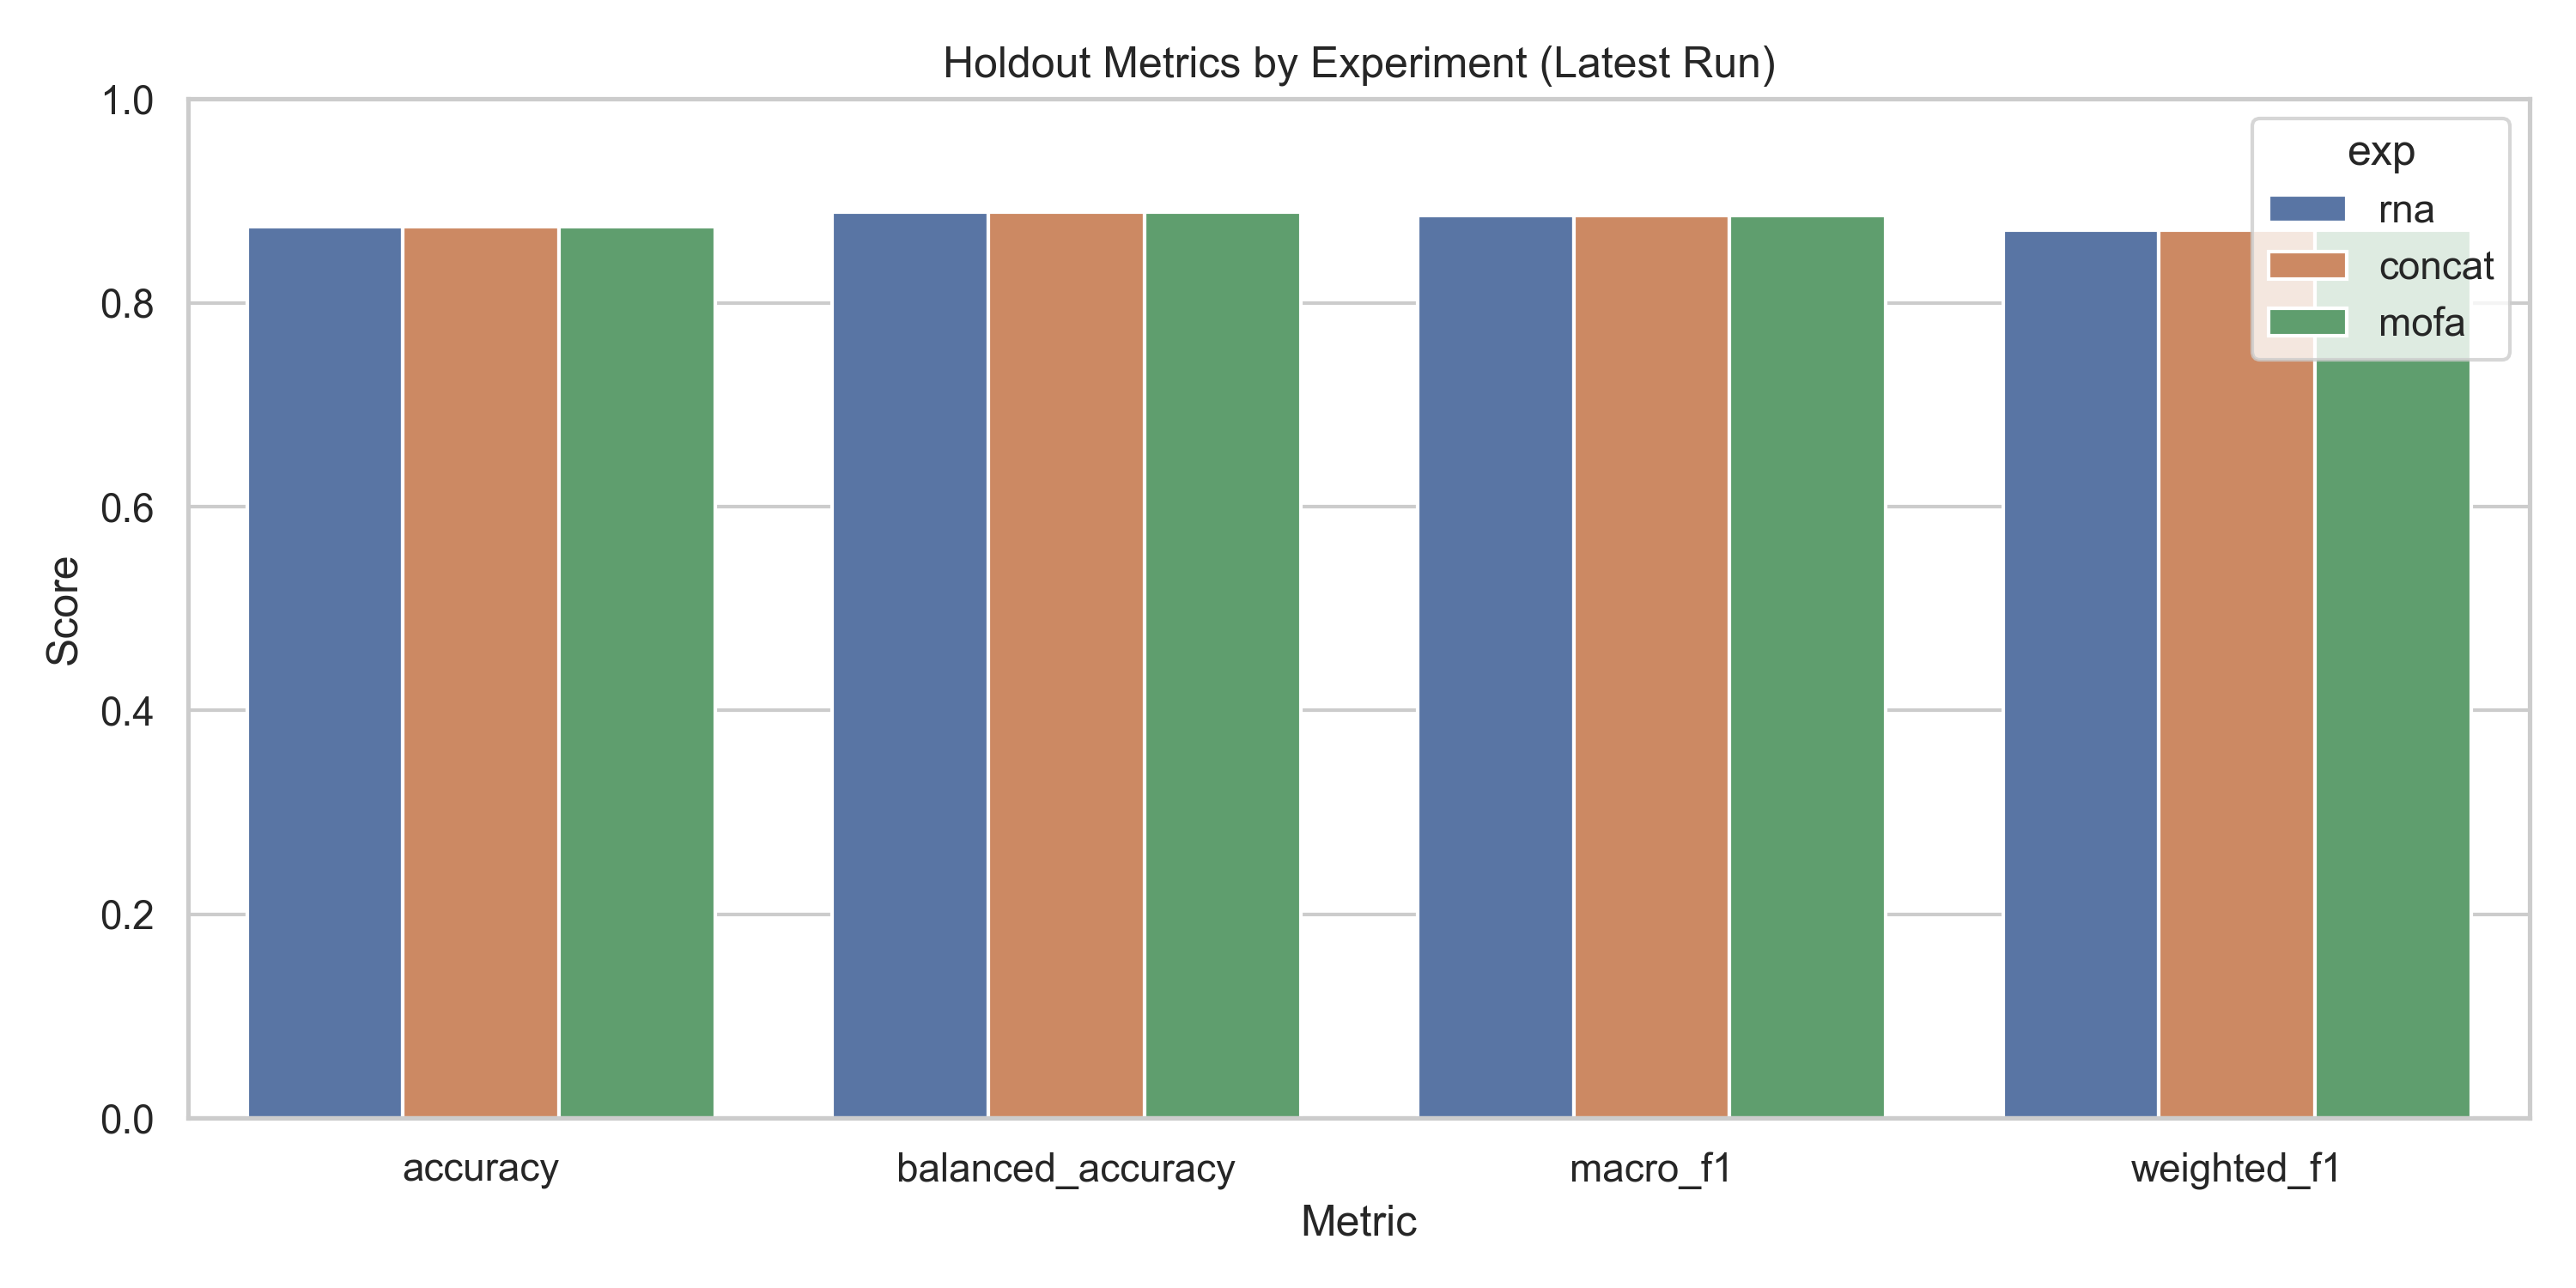
\includegraphics[width=0.92\linewidth]{../../outputs/figures/real_holdout_metrics.png}
\caption{基于真实日志的 holdout 多指标对比图。该图展示各实验在 accuracy、balanced accuracy、macro-F1 与 weighted-F1 上的最新结果。}
\label{fig:real_holdout_metrics}
\end{figure}

\begin{figure}[H]
\centering
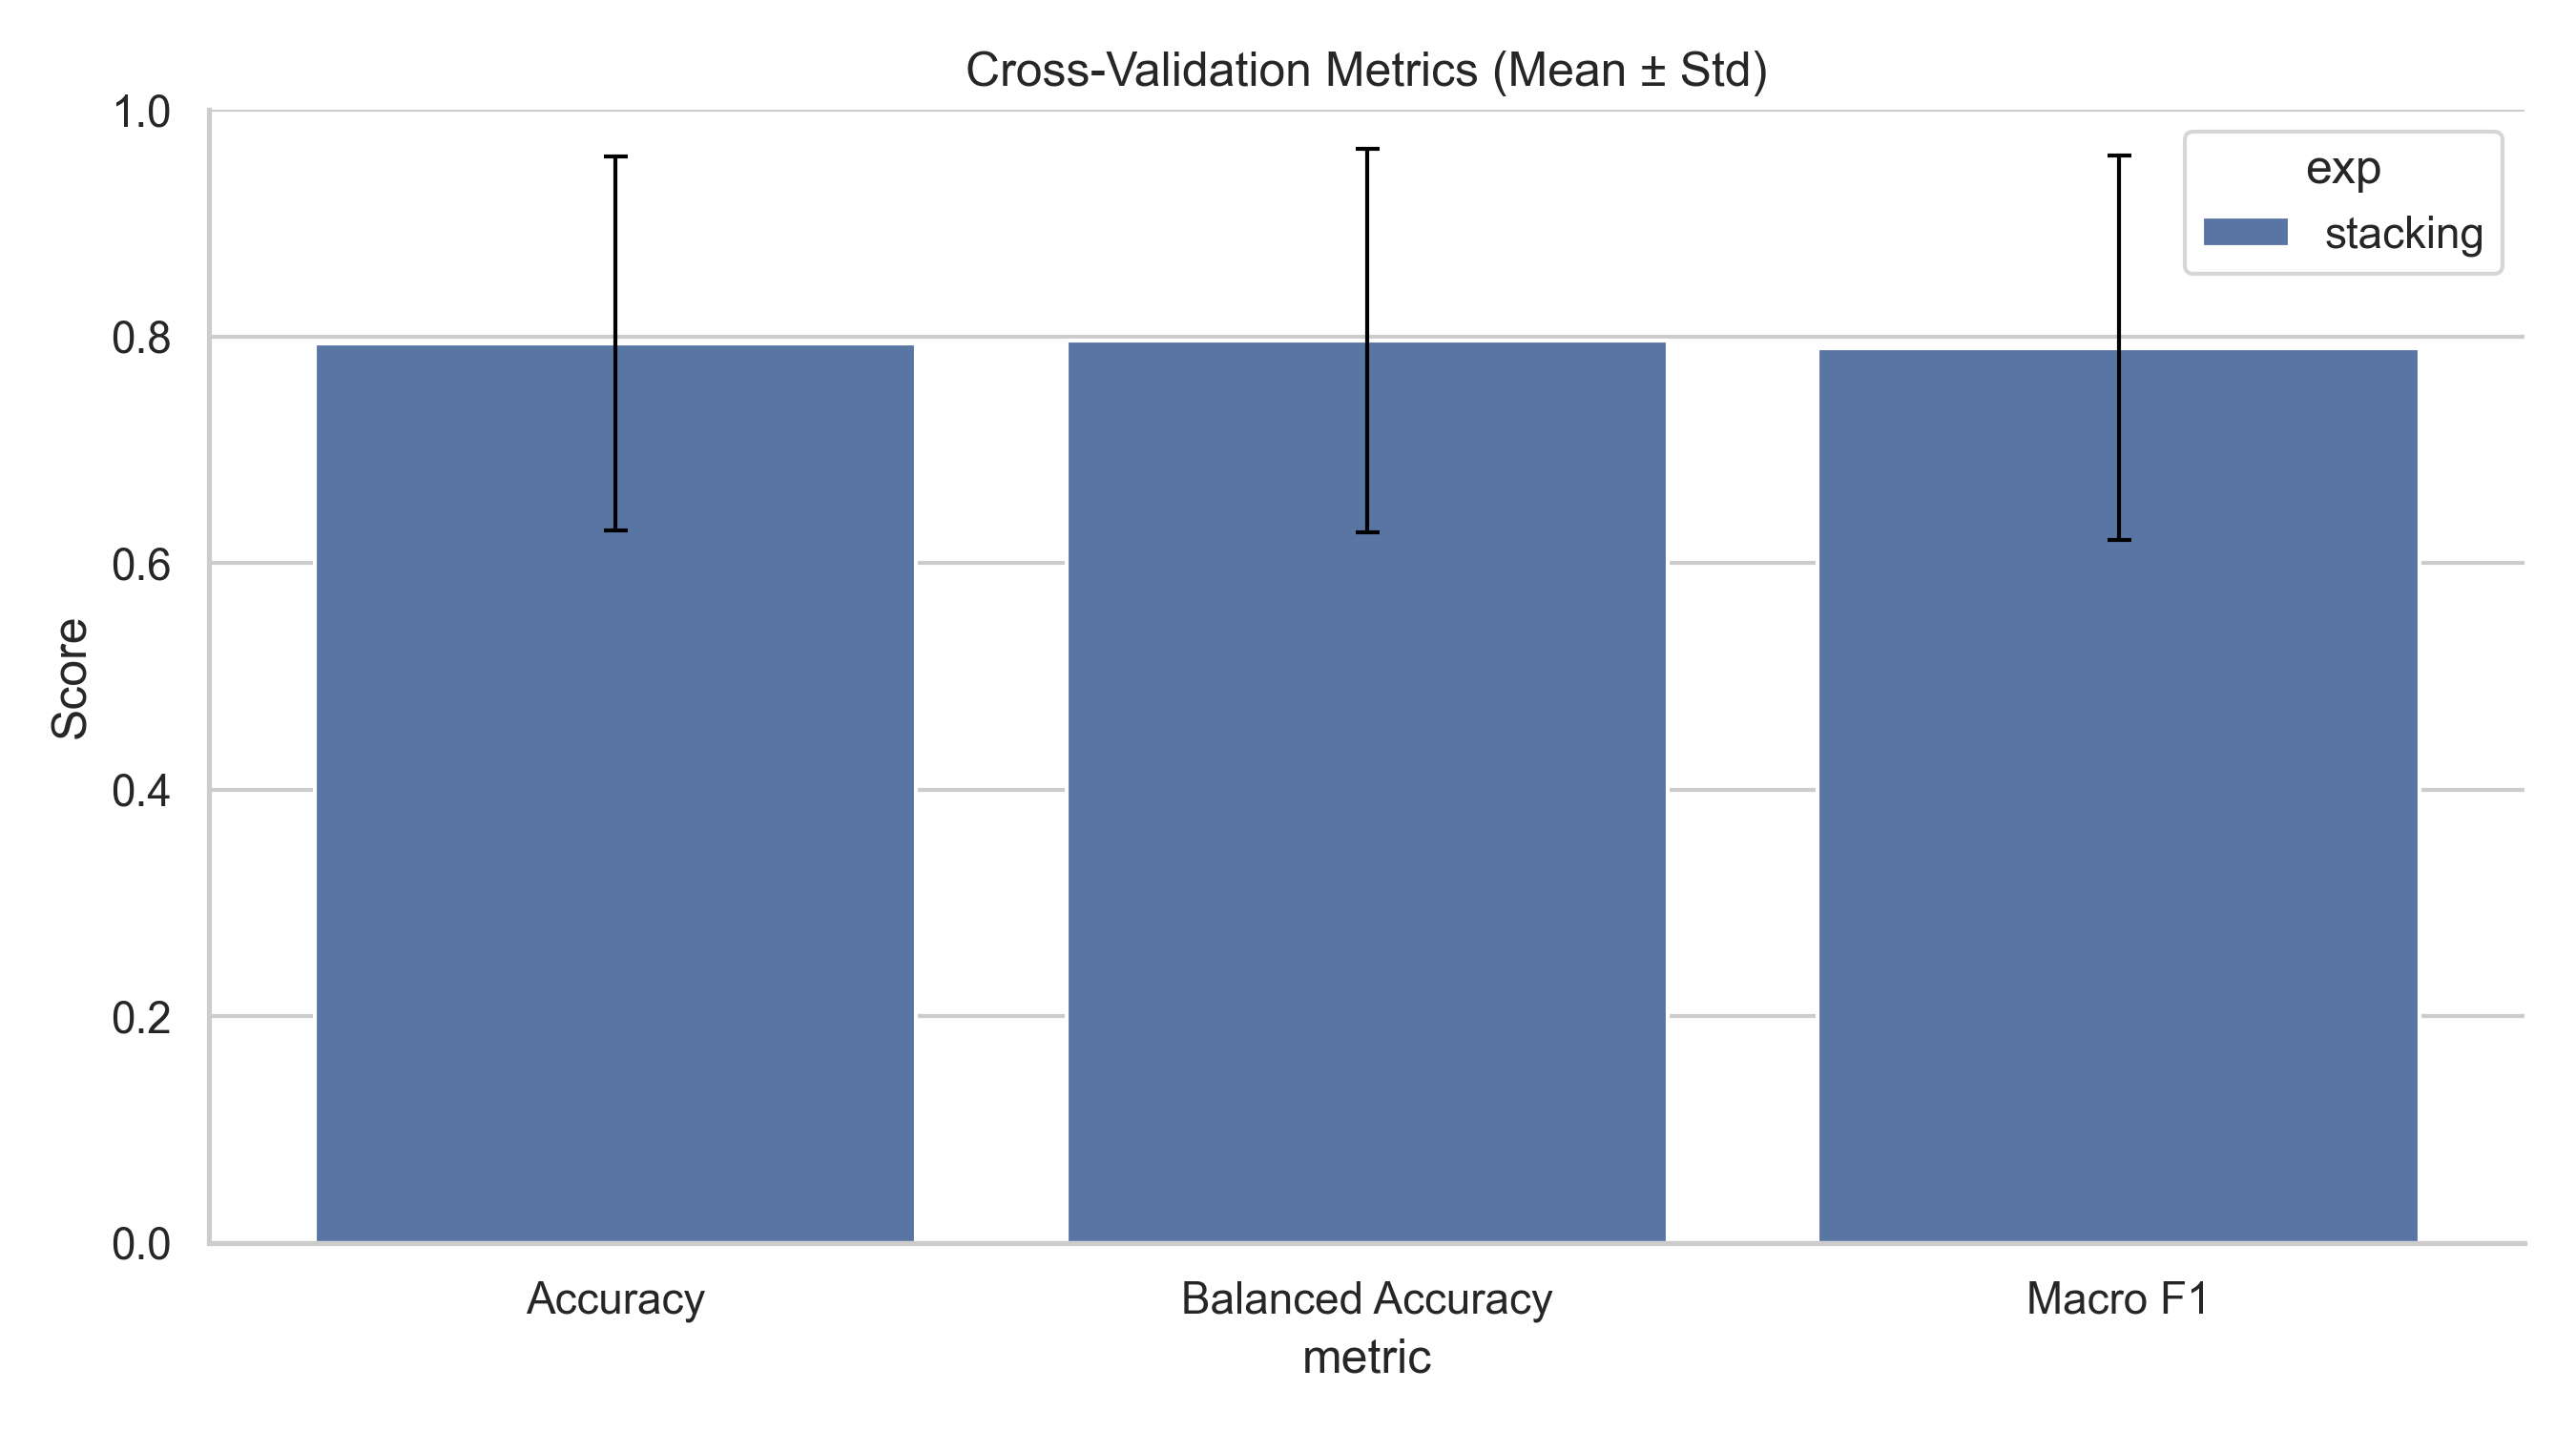
\includegraphics[width=0.92\linewidth]{../../outputs/figures/real_cv_metrics_errorbar.png}
\caption{基于真实日志的交叉验证结果（均值$\pm$标准差）。该图用于直观比较模型性能中心与波动幅度。}
\label{fig:real_cv_metrics}
\end{figure}

\begin{figure}[H]
\centering
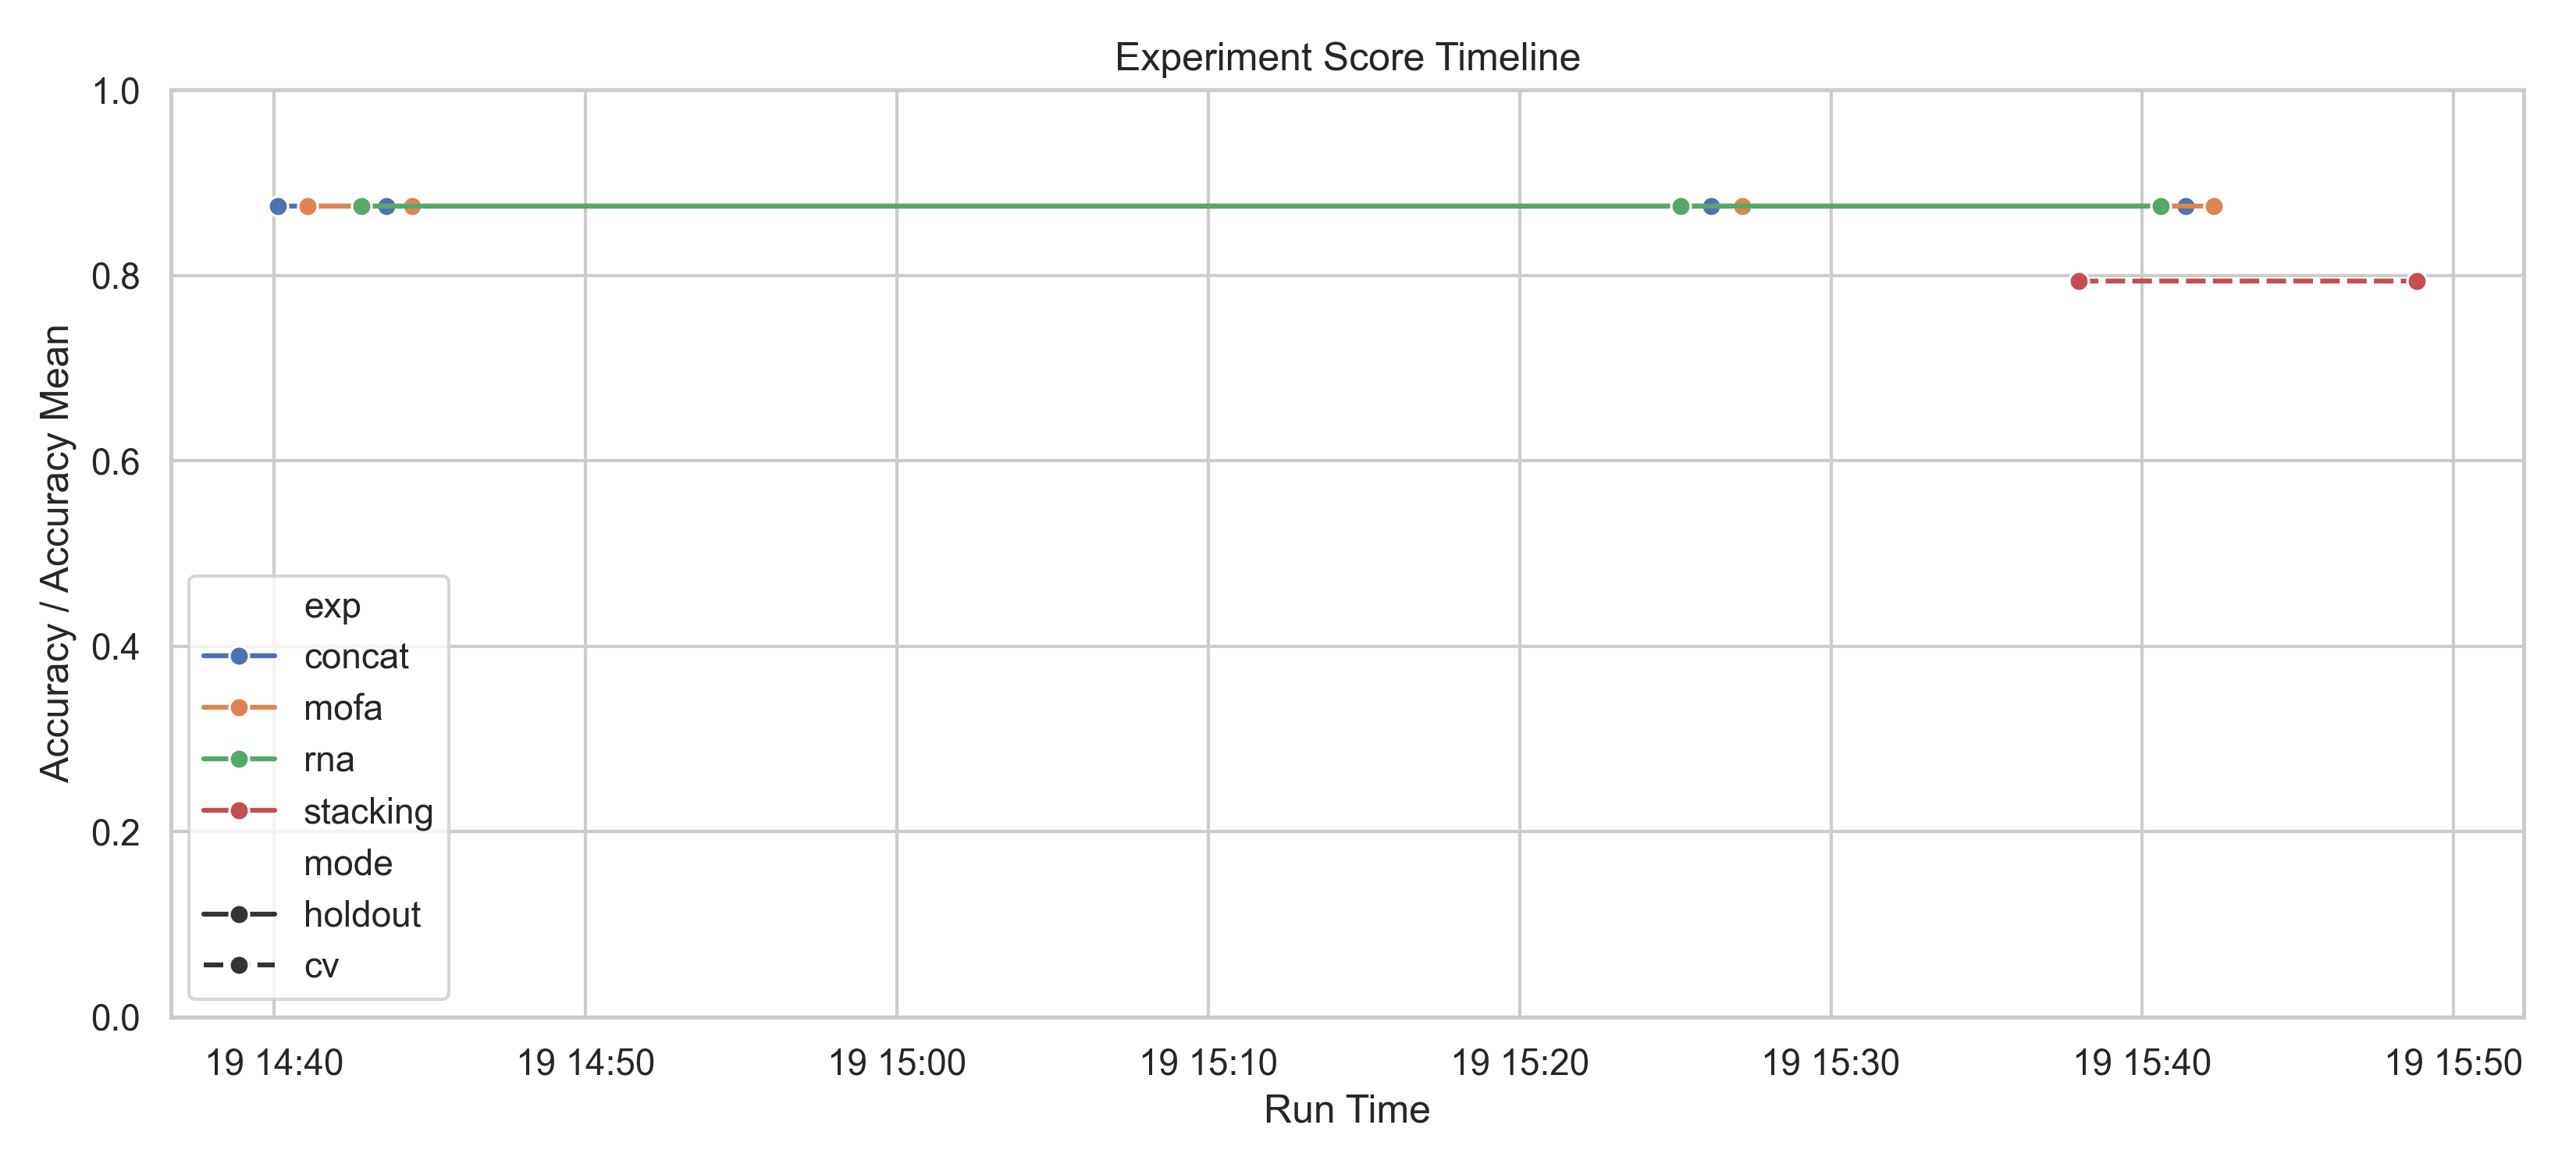
\includegraphics[width=0.92\linewidth]{../../outputs/figures/real_score_timeline.png}
\caption{实验结果时间线。该图展示不同实验在不同时间点的性能变化，用于排查回归问题与版本迭代影响。}
\label{fig:real_score_timeline}
\end{figure}

\begin{figure}[H]
\centering
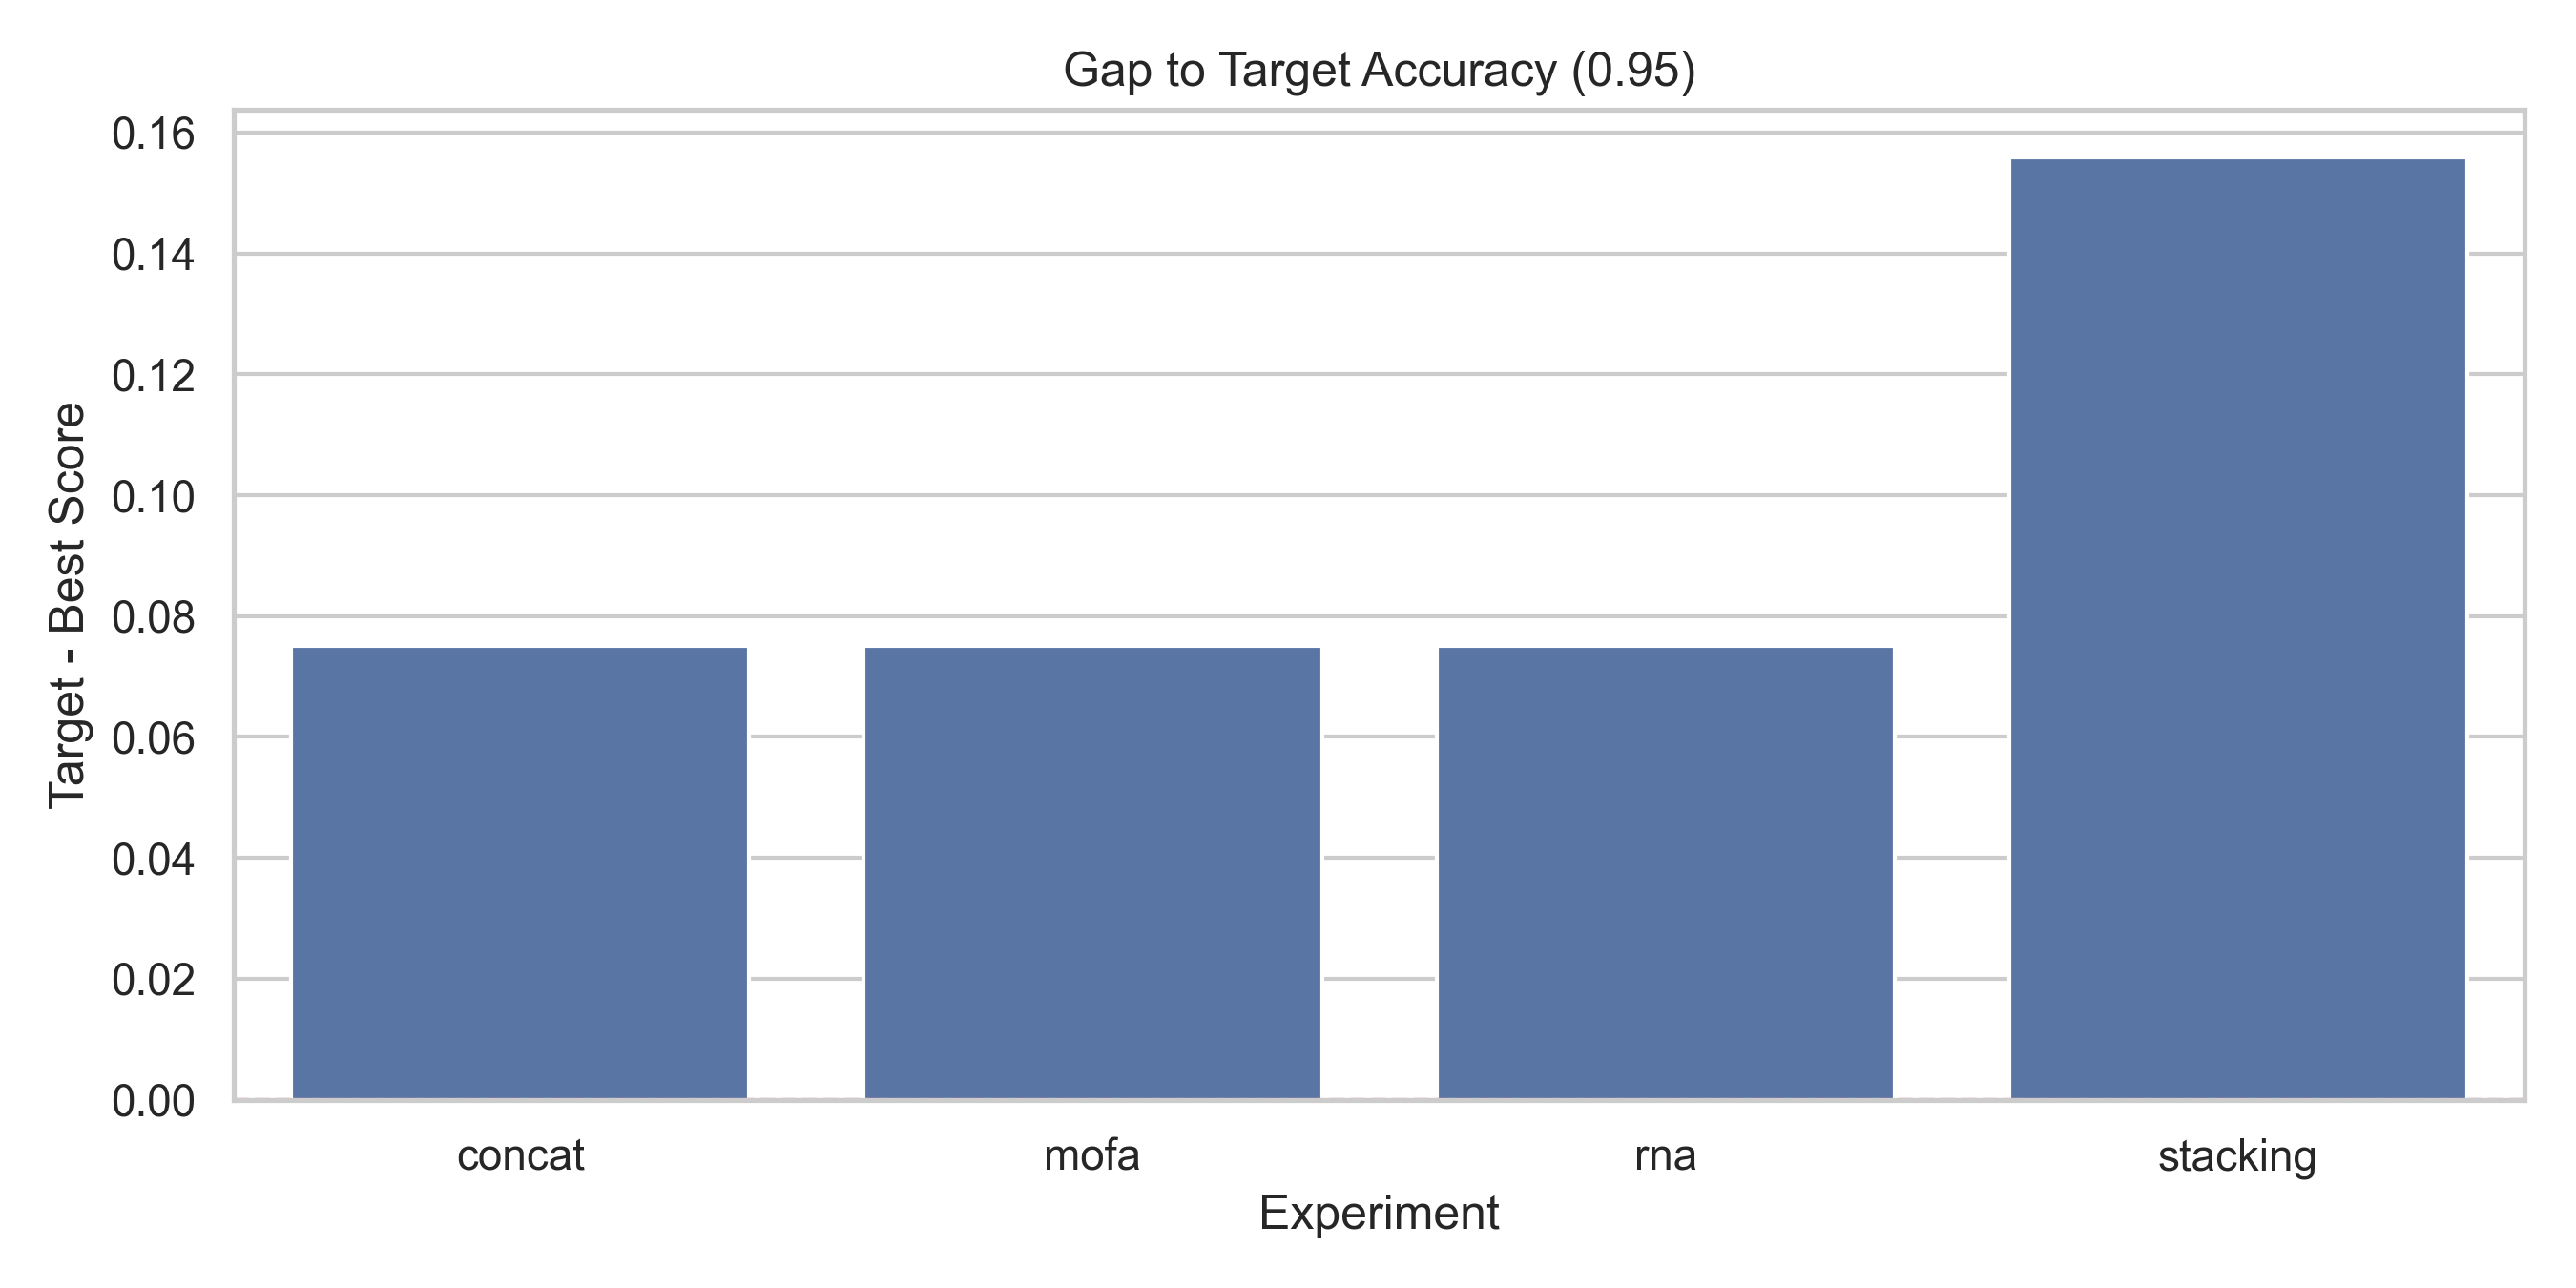
\includegraphics[width=0.85\linewidth]{../../outputs/figures/real_target_gap.png}
\caption{与目标准确率（0.95）的差距分析。柱值越接近 0 表示越接近目标，负值表示已超过目标。}
\label{fig:real_target_gap}
\end{figure}

\subsection{图表证据链解释}

上述四张图构成“结果可复核”证据链：
\begin{enumerate}
	\item \textbf{横向比较}：通过 holdout 与 CV 图分别呈现不同评估口径下的模型差异；
	\item \textbf{不确定性}：通过误差线显式报告方差，避免只看单次高分；
	\item \textbf{时间一致性}：通过时间线图核验结果是否出现异常漂移；
	\item \textbf{目标导向}：通过目标差距图量化当前最优结果与 ACC=0.95 的距离。
\end{enumerate}

这种写法更符合期刊审稿对“可追溯、可重复、可解释”三项要求。

\subsection{模板图与扩展分析说明}

项目中仍保留部分高级图（如特征重要性、超参数敏感性、鲁棒性模板图），其作用是提供后续扩展分析模板，不作为当前稿件的主证据。后续完成多随机种子与外部验证后，可将模板图替换为对应的真实统计图后再进入正文主结果。
